\section{Method}
\label{sec:method}

\subsection{Problem, notation and validity masks}
\label{sec:method-problem}

A pair consists of a query video $A$ and a reference video $B$ with fixed pre-extracted
ISC descriptors~\cite{yokoo2021,douze2021isc}
\begin{equation}
F_A\in\mathbb{R}^{M\times d},\qquad F_B\in\mathbb{R}^{N\times d},\qquad d=256,
\end{equation}
where $i\in\{0,\dots,M-1\}$ and $j\in\{0,\dots,N-1\}$ are \emph{feature indices}. A row is
valid when it is non-empty, finite and has norm above $\varepsilon=10^{-8}$:
\begin{equation}
\begin{aligned}
m_i^A&=\mathbf{1}\!\left[\operatorname{finite}(F_{A,i})\land\lVert F_{A,i}\rVert_2>\varepsilon\right],\\
\fA{i}&=\begin{cases}F_{A,i}/\lVert F_{A,i}\rVert_2,&m_i^A=1,\\ \mathbf{0},&m_i^A=0.\end{cases}
\end{aligned}
\end{equation}
where $\operatorname{finite}$ requires every component to be finite; the norm is
computed in a precision that avoids overflow. Feature files are checked finite at load, the
search and tube stages share the same threshold, and segment extraction consumes the
resulting node-valid mask. Define $m_j^B,\fB{j}$ analogously. Cosine similarity is defined only between valid rows:
\begin{equation}
\Sim_{ij}=\begin{cases}\langle \fA{i},\fB{j}\rangle,&m_i^A=m_j^B=1,\\-\infty,&\text{otherwise.}\end{cases}
\label{eq:sim}
\end{equation}
We keep explicit video superscripts throughout; an unlabelled
$\langle \bar f_i,\bar f_j\rangle$ would be ambiguous when the two videos are indexed
independently. An invalid row is never a match node, never contributes evidence, and cannot
start or end a prediction.

The output is a set of half-open interval pairs
\begin{equation}
\begin{aligned}
\mathcal{Y}=\{&(a_s,b_s,a_e,b_e,q)\mid 0\le a_s<a_e\le M,\\
&0\le b_s<b_e\le N,\;q\in\mathbb{R}\},
\end{aligned}
\label{eq:output}
\end{equation}
with uncalibrated score $q$, not a probability. Coordinates are feature indices; converting
them to seconds or original-video frame numbers requires a verified timestamp map, which the
current draft does not establish. We never call a feature index a second or a source-video frame.

\begin{figure*}[t]
  \centering
  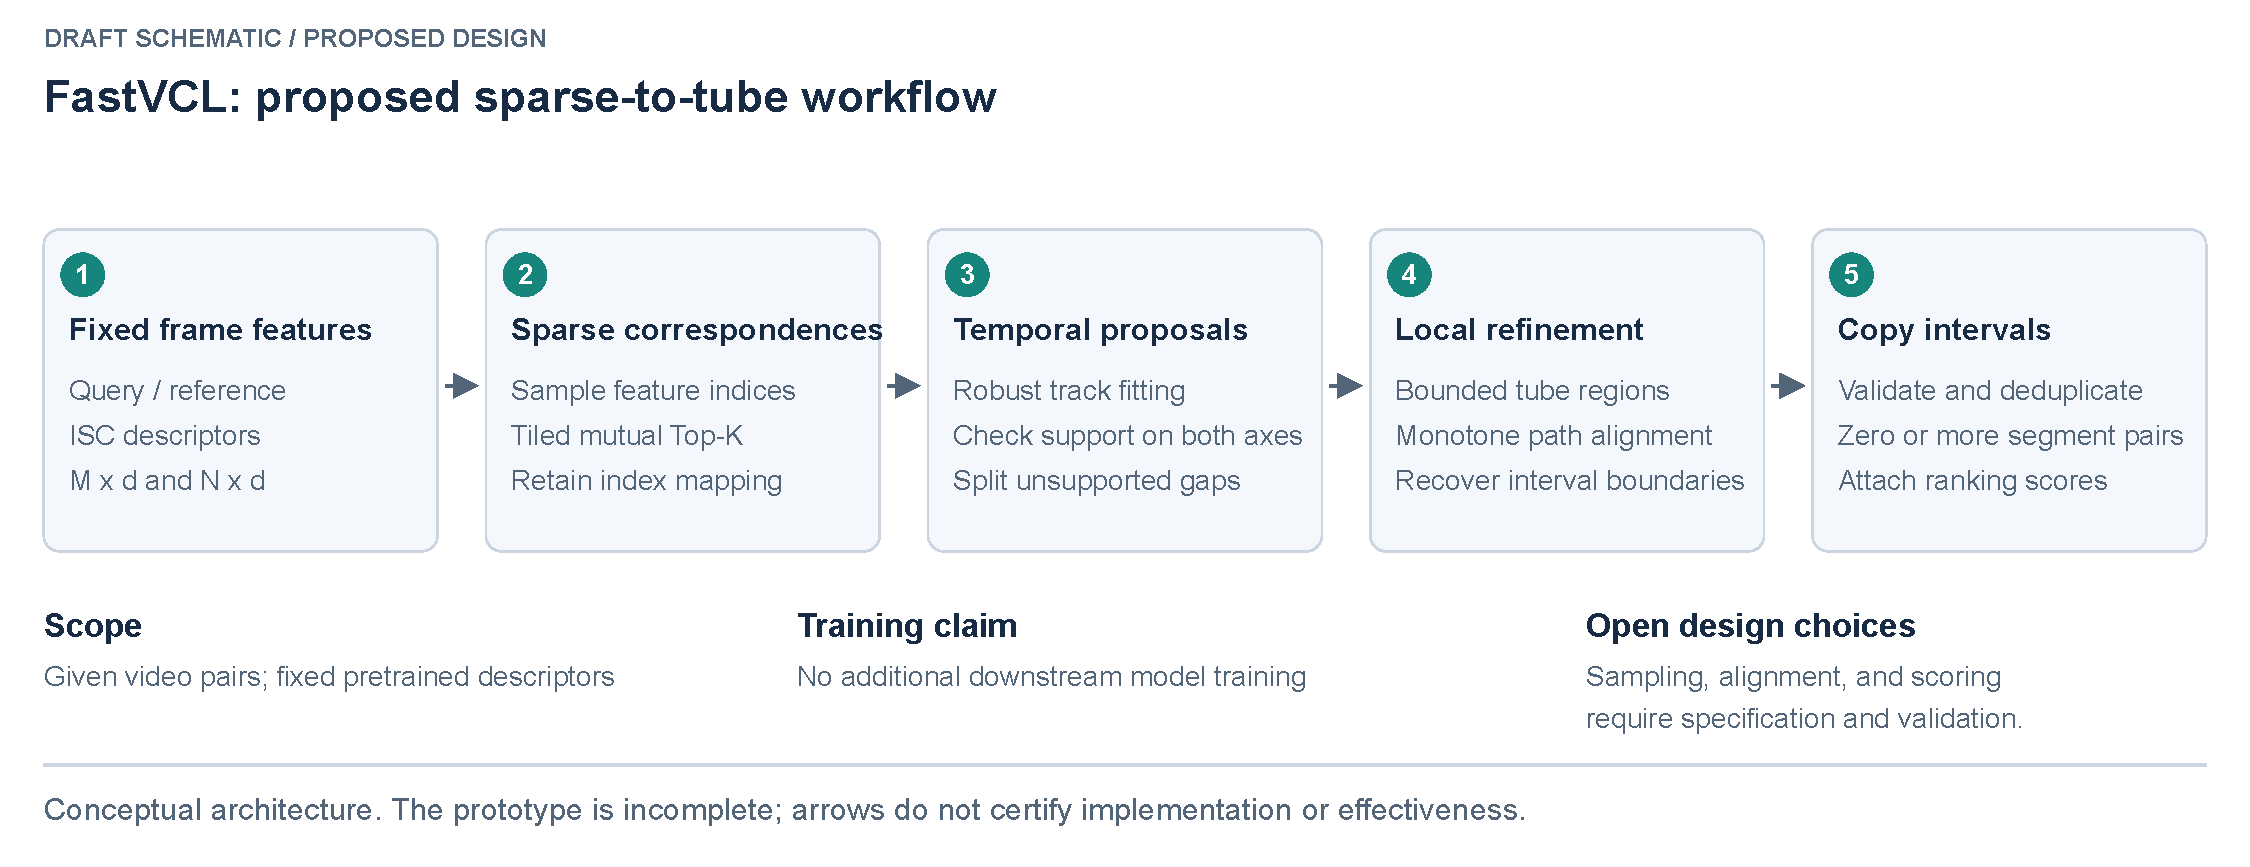
\includegraphics[width=\textwidth]{figures/fig_2_framework.pdf}
  \caption{\textbf{FastVCL framework (proposed method).}
  Normalized fixed features produce sparse mutual anchors, robust temporal tracks and finite
  tubes. Full-resolution descriptors (blue dashed connection) are reused for in-tube local
  DP, segment extraction and de-duplication. The lower row adds proposed frame-based
  verification, named \texttt{seltive model} (Section~\ref{sec:method-selective}); its policies
  remain unspecified and no result includes it. Matrices, paths and intervals are schematic.
  The zero-floored DP differs from the current prototype.}
  \label{fig:framework}
\end{figure*}

\subsection{Sparse correspondence proposals}
\label{sec:method-sparse}

\paragraph{Sampling grids.}
A plan $g=(s_A^g,s_B^g,p_A^g,p_B^g)\in\Grid$ has strides $s_A^g,s_B^g\ge1$ and phases
$0\le p_A^g<s_A^g$, $0\le p_B^g<s_B^g$. Its valid sampled sets are
\begin{align}
I_A^g&=\{p_A^g+k s_A^g:k\ge0\}\cap\{i:m_i^A=1\},\\
I_B^g&=\{p_B^g+k s_B^g:k\ge0\}\cap\{j:m_j^B=1\},
\end{align}
and only $I_A^g\times I_B^g$ is scored inside plan $g$.

\paragraph{Mutual Top-$K$ anchors.}
Let $\operatorname{TopK}^{(K)}_{B,g}(i)\subseteq I_B^g$ contain the $\min(K,|I_B^g|)$ elements largest
under the total order $(i,j')\succ(i,j)$ iff $\Sim_{ij'}>\Sim_{ij}$, or
$\Sim_{ij'}=\Sim_{ij}$ and $j'<j$. Ties are resolved by the smaller original index,
deterministically and identically in both directions. The plan-level set is
\begin{equation}
\begin{aligned}
\Anch_g=\Big\{&(i,j)\in I_A^g\times I_B^g:\;
j\in\operatorname{TopK}^{(K)}_{B,g}(i),\\
&i\in\operatorname{TopK}^{(K)}_{A,g}(j),\;
\Sim_{ij}\ge\tau\Big\}.
\end{aligned}
\label{eq:anchors}
\end{equation}
Bidirectional membership removes one-sided matches; it does not guarantee removal of
repeated-texture matches. The threshold $\tau$ removes low-cosine anchors.

\paragraph{Merging plans.}
Across plans, anchors are merged \emph{by original coordinate}:
\begin{equation}
\Anch=\operatorname{Cap}_{C_{\max}}\!\left(\operatorname{Dedup}_{(i,j)}
\bigcup_{g\in\Grid}\Anch_g\right),
\label{eq:merge}
\end{equation}
where $\operatorname{Dedup}_{(i,j)}$ keeps one copy per coordinate with the largest cosine and
$\operatorname{Cap}_{C_{\max}}$ keeps the $C_{\max}$ highest scores (ties by smaller index).
Without coordinate de-duplication one physical correspondence could support several RANSAC
inliers and inflate a track's evidence.

\paragraph{Sampling facts that constrain the experiments.}
Zero-phase grids are nested ($I^{8}\subset I^{4}\subset I^{2}$): a coarser grid adds no
coordinate but changes each row's Top-$K$ competition, so a multi-scale run must be compared
with a single fine grid at an equal executed budget. Independent phase pairs differ from
synchronous shifts $(p,p)$ and tile the two-dimensional offset. For one stride-$s$ grid, $h$
distinct A anchor times span at least $(h-1)s$ indices, so a shorter copy cannot supply them
wholly within itself; outside anchors, tube extension or merged phases may still produce a
candidate overlapping that copy, and this is not an impossibility theorem. Top-$K$ partners
share a time and are not independent support. The supplement records the derivations and
the 64$\times$64 budget counts.

\subsection{Robust temporal tracks with dual-axis validation}
\label{sec:method-tracks}

\paragraph{Model and fitting.}
Each local correspondence is modelled as
\begin{equation}
j\approx\alpha_r i+\beta_r,\qquad \alpha_r\in[\alpha_{\min},\alpha_{\max}]\subset(0,\infty).
\label{eq:line}
\end{equation}
The slope is an index-step ratio; it equals a playback-speed ratio only when both videos have
the same constant sampling rate. RANSAC repeatedly draws two anchors at distinct A
coordinates, computes $(\alpha,\beta)$, counts inliers under
\begin{equation}
|j-(\alpha i+\beta)|\le\epsilon_B,
\label{eq:inlier}
\end{equation}
and keeps the best hypothesis. The draw is deterministic given a per-pair seed derived from a
cryptographic hash of the structured pair identifier, so resumes and reruns see the same
hypotheses. Model inliers are removed provisionally; if every split run fails re-validation,
they are restored so another hypothesis can explain them. This allows several copies between
the same pair.

\paragraph{Dual-axis re-validation.}
Each run $\Track_r$ is refitted and accepted only if
\begin{equation}
\alpha_{\min}\le\alpha_r\le\alpha_{\max},\qquad
\max_{(i,j)\in\Track_r}|j-(\alpha_r i+\beta_r)|\le1.5\,\epsilon_B,
\label{eq:recheck}
\end{equation}
\begin{equation}
|\pi_A(\Track_r)|\ge h_A,\qquad|\pi_B(\Track_r)|\ge h_B,
\label{eq:support}
\end{equation}
\begin{equation}
\begin{aligned}
\max\pi_A(\Track_r)-\min\pi_A(\Track_r)&\ge L_{\min}^A,\\
\max\pi_B(\Track_r)-\min\pi_B(\Track_r)&\ge L_{\min}^B .
\end{aligned}
\label{eq:span}
\end{equation}
Checking support after the refit matters: a refit can collapse to a degenerate line that
passes the original inlier test. Requiring both axes rejects a track that is long in query time
but pinned to one reference instant, the signature of a static logo or repeated still.

\paragraph{Gap splitting.}
Sort inliers by $i$ and split between consecutive pairs whenever
\begin{equation}
\begin{aligned}
&i_{(t+1)}-i_{(t)}>g_A,\quad\text{or}\quad
j_{(t+1)}-j_{(t)}>g_B,\\
&\text{or}\quad j_{(t+1)}-j_{(t)}<-g_{\mathrm{back}} .
\end{aligned}
\label{eq:gapsplit}
\end{equation}
Each run is re-validated by \eqref{eq:recheck}--\eqref{eq:span}. The gap rules separate unsupported spans and large backward steps; they do not
guarantee that later tube extensions or extracted intervals remain disjoint. Splitting can create several runs, but re-validation may reject some or all of them;
the number of accepted proposals can increase or decrease. The supplement illustrates the
anchor-to-tube construction on hand-chosen coordinates; it is not a real-pair result.

\subsection{Finite tubes}
\label{sec:method-tube}

For a track $r$ with support $[i^r_{\min},i^r_{\max}]$ and
$c_r(i)=\operatorname{round}(\alpha_r i+\beta_r)$ (ties to even),
\begin{equation}
\begin{aligned}
\ell_r&=\max(0,\,i^r_{\min}-e_A),\quad
u_r=\min(M,\,i^r_{\max}+1+e_A),\\
L_r&=u_r-\ell_r,\\
\Tube_r&=\{(i,j):\ell_r\le i<u_r,\\
&\qquad j=c_r(i)+\delta,\;-w_r\le\delta\le w_r,\;0\le j<N\}.
\end{aligned}
\label{eq:tube}
\end{equation}
The extension $e_A$ moves the search along the trajectory beyond the anchors; the half-width
$w_r$ absorbs jitter and small speed changes. The tube has at most $L_rW_r$ cells with
$W_r=2w_r+1$.

Two limitations follow from the definition. Refinement can only act inside
$\bigcup_r\Tube_r$: a copy with no fitted track is unreachable regardless of alignment quality.
And $e_A$ is a search extension, not a boundary estimate; endpoints come from matched nodes,
never from the window edge. A tube built from ground-truth boundaries answers a different
question and is used only as a separately labelled oracle diagnostic. Here $e_A$ and $w_r$ are
constants; calling them uncertainty-adaptive would be false.

\subsection{In-tube local alignment}
\label{sec:method-dp}

\paragraph{Proposed recurrence.}
For $(i,j)\in\Tube_r$, let $r_{ij}=\Sim_{ij}-\tau_{\mathrm{align}}$, with
$r_{ij}=-\infty$ if either row is invalid. With
$\Pred_r(i,j)=\{(i-\Delta i,j-\Delta j)\in\Tube_r:(\Delta i,\Delta j)\in\Step\}$ and
$\Step=\{(1,1),(1,2),(2,1)\}$, the proposed score is
\begin{equation}
\begin{aligned}
H_{ij}=\max\Big(&0,\;r_{ij},\\
&\max_{\substack{(u,v)\in\Pred_r(i,j)\\ H_{uv}>0}}
\big[H_{uv}+r_{ij}-\lambda_{\mathrm{gap}}\,g(i-u,j-v)\big]\Big),
\end{aligned}
\label{eq:localdp}
\end{equation}
with $g(\Delta i,\Delta j)=\Delta i+\Delta j-2$. Equation~\eqref{eq:localdp} is a
Smith--Waterman-style local alignment~\cite{smith1981} with the stated restricted steps;
it is not the canonical insertion/deletion recurrence. Invalid or previously blocked cells
have $H=0$, no predecessor and cannot be used as match nodes. The zero is a
\emph{restart}: a cell may always abandon a bad prefix. A weak frame lowers the accumulated
score but does not by itself force a restart, so a short weak stretch is bridged while the
score remains positive; the floor only discards a path once its evidence is exhausted. This is
the intended protection when $e_A$ includes a weak non-copy prefix; its empirical effect
remains to be tested.

\paragraph{Backtrace and intervals.}
Let $(i^\star,j^\star)=\argmax H_{ij}$ if $H_{i^\star j^\star}>0$. We follow the predecessor
that attained the maximum until reaching a restart or a cell with no legal predecessor. The
visited nodes, ordered by $i$, define
\begin{equation}
[a_s,a_e)=[i_{\text{first}},\,i_{\text{last}}+1),\qquad
[b_s,b_e)=[j_{\text{first}},\,j_{\text{last}}+1),
\label{eq:interval}
\end{equation}
which is half-open and integer by construction. A non-positive cell is never a valid start. For tied positive maxima choose the smallest
$(i,j)$; for tied transitions prefer a restart, then the stated step order. This deterministic
rule belongs to the proposed specification.

\paragraph{Restart semantics and segment extraction.}
The prototype instead keeps a legal continuation even when negative: a cell with a legal
predecessor never restarts, so a negative cell cannot start a traceback but a later strong
cell inherits its deficit. On a one-cell-wide band, a long weak prefix can then prevent a
later copy from attaining a positive score; a second copy can inherit a preceding gap's
negative score. These constructed cases and their exact scores are shown in the supplement.
E3 compares both rules on identical tubes; neither a toy example nor the zero-floor
principle establishes a benchmark improvement.

For the proposed output rule, clamp path cosines below zero, then average over a centered
window of up to three matched nodes with edge padding. Keep nodes at or above
$\tau_{\mathrm{seg}}$. Consecutive strong nodes belong to the same segment only if
$i_{t+1}-i_t-1\le g_{\mathrm{low}}$, counting intervening original A indices. Trim to the
first and last strong nodes, then read endpoints by \eqref{eq:interval}. Apply minimum
durations on both axes and minimum distinct anchor support within the segment. The proposed
endpoints have no additional margin; the prototype applies a margin counted in matched path
rows (default 2), not in feature indices, and counts stored A-anchor entries rather than
distinct times. Both differences are recorded in the supplement.

After each positive path, block only its matched cells and recompute the DP, up to $P_r$
attempts, including attempts whose extracted segments are rejected. Blocking a whole row or
column would remove other copies. Stop before backtrace if no positive unblocked path exists.
This greedy extraction does not guarantee the globally optimal set of paths.

\subsection{Multi-segment output, score and de-duplication}
\label{sec:method-segments}

Two interval pairs are near-duplicates when
\begin{equation}
\begin{aligned}
&\min\big(\IoU_1([a_{s,1},a_{e,1}),[a_{s,2},a_{e,2})),\\
&\qquad\IoU_1([b_{s,1},b_{e,1}),[b_{s,2},b_{e,2}))\big)\ge\theta_{\mathrm{dedup}} .
\end{aligned}
\label{eq:miniou}
\end{equation}
The minimum, not an A-only or area IoU, is deliberate. If the same query interval
$[a_s,a_e)$ is copied at two reference times, $\IoU_A=1$ but $\IoU_B=0$, so both copies are
kept; an A-only rule would delete one. A two-dimensional area-IoU rule also keeps this
disjoint-reference example, so the example alone does not establish an advantage over that rule. The rule is for de-duplication, not evaluation; the
official metric uses a product (Section~\ref{sec:exp-metric}).

The confidence is an uncalibrated combination of mean smoothed path similarity and anchor
support,
\begin{equation}
q=0.7\cdot\operatorname{clip}(\bar s,0,1)+0.3\cdot
\min\!\left(1,\frac{n_A^{\mathrm{seg}}}{\max(1,\,L_A/\bar\Delta_A)}\right),
\label{eq:score}
\end{equation}
where $\bar s$ is the mean smoothed value over retained path nodes, $L_A=a_e-a_s$,
$n_A^{\mathrm{seg}}$ is the number of distinct A times among track anchors whose A and B
coordinates both lie inside the segment, and $\bar\Delta_A$ is the median positive spacing
of distinct track A times (fallback 4 when fewer than two exist). Distinct support avoids
rewarding repeated Top-$K$ partners as independent times. The prototype counts stored
A-anchor entries over the A interval only, so Top-$K>1$ can change its support term. This
proposed rule must be reconciled with the prototype before evaluation. Greedy de-duplication
visits decreasing $q$, breaking ties by start coordinates and then collection order; apply
the configured segment cap. The confidence threshold is applied by the evaluation protocol,
not by the core pipeline, and its mode is declared with the run. Scores are not calibrated
across methods.

An empty list is a legitimate prediction for a negative or low-confidence pair
(\textsc{empty}). A missing file, exception, timeout or out-of-memory event is
\textsc{error}/\textsc{skipped} and is never rewritten as an empty list; doing so would change
the denominators in Section~\ref{sec:exp-metric}.

\subsection{Proposed selective verification: \texttt{seltive model}}
\label{sec:method-selective}
Figure~\ref{fig:framework} includes an optional JEV visual-copy verification branch under
its requested name, \texttt{seltive model}. It consumes selected candidate intervals and
matched indices together with original A/B frame context. It therefore requires a verified
feature-index-to-frame map and additional visual input beyond the fixed ISC descriptors.
A proposed verifier returns \texttt{COPY}, \texttt{NOT\_COPY} or \texttt{UNCERTAIN}; an
unselected candidate, uncertain verdict or failed call retains the core prediction.
Selection, model backend and the action on decisive verdicts remain unspecified. We do not
assign an unvalidated deletion or score-update rule.

The extension cannot recover a copy absent from its candidate pool and is excluded from
Algorithm~\ref{alg:fastvcl} and the core H1--H3 comparison. E6 must compare core-only,
random selection and selective verification on the same pool and call budget, report recall
loss and false alarms, and add frame acquisition, model calls, failures, retries and fusion
to the cost. No backend, benefit or downstream training status is established.

\subsection{Algorithm and complexity}
\label{sec:method-complexity}

Algorithm~\ref{alg:fastvcl} summarizes one pair. Complexity must be stated twice: for the
arithmetic the design intends and for the scanning an implementation performs. Conflating them
is how a memory saving is misreported as an algorithmic speed-up.

\paragraph{Coarse stage.}
The number of scored grid pairs is
\begin{equation}
Q^{\mathrm{grid}}_{\mathrm{coarse}}
=\sum_{g\in\Grid}|I_A^g|\,|I_B^g|
\approx MN\sum_{g\in\Grid}\frac{1}{s_A^g s_B^g}.
\label{eq:qcoarse}
\end{equation}
With all rows valid and fixed strides this is $\Theta(MN)$ (an $O(MN)$ upper bound
with masks): the constant shrinks, the order does not. Three
properties must be kept apart: not storing the full $M\times N$ matrix (memory, via tiling
and streaming); keeping few anchors (output sparsity, $|\Anch|\ll MN$); and performing
sub-quadratic arithmetic (false for fixed strides). If forward and backward Top-$K$ scans are
evaluated separately, the executed dot-product count is about $2Q^{\mathrm{grid}}_{\mathrm{coarse}}$
plus tie work; efficiency comparisons report that executed count.

\paragraph{Refinement stage.}
With direct offset addressing, the predecessor under $(\Delta i,\Delta j)$ has band-relative
column $\delta_u=(j-\Delta j)-c_r(i-\Delta i)$, computed in $O(1)$; one dynamic program costs
\begin{equation}
O\!\left(L_rW_r|\Step|\right)=O(L_rW_r)
\label{eq:dpideal}
\end{equation}
per path, and $O(P_rL_rW_r)$ for $P_r$ attempts, plus $O(d\,L_rW_r)$ to compute the band once.
If the implementation scans all $W_r$ columns of the predecessor row for non-diagonal steps,
the per-cell cost is $O(W_r)$ and the per-tube cost becomes
\begin{equation}
O\!\left(P_rL_rW_r^{\,2}\right).
\label{eq:dpscan}
\end{equation}
Both bounds are reported, and the measured one is named in the timing results.

\paragraph{Whole-pipeline time and memory.}
In addition to normalization and dot products, account for tiled Top-$K$ selection,
$O(RI|\Anch|)$ RANSAC hypothesis scoring for at most $R$ rounds and $I$ trials per round,
refits/sorting, traceback and worst-case $O(C^2)$ greedy de-duplication of $C$ segments.
The DP bound alone is not the pipeline bound. Resident input is $O((M+N)d)$. Beyond it,
coarse storage includes the tile ($B_A B_B$ cells), retained Top-$K$ lists
($K(n_A+n_B)$ entries for sampled lengths $n_A,n_B$), and anchors; sequential refinement
requires $O(\max_r L_rW_r)$ tables. Peak RSS must also include retained candidates and
runtime objects. Overlapping tubes duplicate work even when processed sequentially.

\begin{algorithm}[t]
\caption{FastVCL: one video pair}
\label{alg:fastvcl}
\begin{algorithmic}[1]
\Require $F_A,F_B$; the configuration of Sections~\ref{sec:method-sparse}--\ref{sec:method-segments}
\Ensure $\mathcal{Y}=\{(a_s,b_s,a_e,b_e,q)\}$
\State compute masks $m^A,m^B$ and unit rows $\fA{i},\fB{j}$
\State $\Anch\gets\emptyset$
\ForAll{plans $g\in\Grid$}
  \State score $I_A^g\times I_B^g$; keep mutual Top-$K$ with $\Sim_{ij}\ge\tau$
  \State $\Anch\gets\Anch\cup\Anch_g$ \Comment{original indices}
\EndFor
\State $\Anch\gets\AnchorCap_{C_{\max}}(\Dedup_{(i,j)}(\Anch))$
\State $\mathcal{R}\gets$ multi-track RANSAC with \eqref{eq:line}--\eqref{eq:span}
\State split every $r\in\mathcal{R}$ by \eqref{eq:gapsplit}; re-validate
\State $\mathcal{C}\gets\emptyset$
\ForAll{tracks $r$}
  \State build $\Tube_r$ by \eqref{eq:tube}; compute valid similarities once
  \For{$p=1$ \textbf{to} $P_r$}
    \State run \eqref{eq:localdp} on unblocked valid cells
    \If{no positive score} \State \textbf{break} \EndIf
    \State backtrace; trim and extract segments $\mathcal C_r$
    \State $\mathcal C\gets\mathcal C\cup\mathcal C_r$
    \State block matched cells, including paths yielding no segment
  \EndFor
\EndFor
\State $\mathcal{C}\gets$ filter by duration/support; score by \eqref{eq:score}
\State $\mathcal{Y}\gets$ score-ordered de-duplication by \eqref{eq:miniou}
\State apply segment cap; write scores \Comment{threshold is declared at evaluation}
\State \Return $\mathcal{Y}$ \Comment{possibly empty}
\end{algorithmic}
\end{algorithm}
